\documentclass[11pt]{exam}
\usepackage[margin=1in]{geometry}
\pagestyle{plain}
\usepackage{amsmath,amsfonts,amssymb,amsthm,enumerate}
\usepackage{multicol}
\usepackage[]{graphicx}
\usepackage{hyperref}
\usepackage{tikz}
\usepackage{pgfplots}
\usepackage{subfigure}
\usepackage[final]{pdfpages}

\addtolength{\footskip}{2\baselineskip} % to lower the page numbers
\title{\vspace{-0.5in} Math 115 Fall 2024 \\ Worksheet 23 -- Section 4.1}
\date{}


% \theoremstyle{definition}
% \newtheorem{problem}{Problem}
\renewcommand{\questionlabel}{\textbf{Problem~\thequestion.}}
%\printanswers

\begin{document}
\maketitle
\vspace{-0.75in}
\section*{Warm-up}
A \textbf{critical point} of $g$ is a point $p$ in the domain of $g$
where $\fillin[g'(p)=0]$ or $\fillin[g'(p) \text{ DNE}]$.
\vskip2ex
\textbf{Note:} ``Critical point'' may refer to just the $x$-value, or to the coordinate pair.
\vskip2ex
A point $p$ in the domain of $g$ where $g(p)\leq g(x)$ for all $x$
near $p$ is a \fillin[local minimum].
\vskip2ex
A point $p$ in the domain of $g$ where $g(p)\geq g(x)$ for all $x$
near $p$ is a \fillin[local maximum].


\vskip2ex
Which of the labeled points in the graph below are critical points? Which are local extrema?
\vspace*{-.4cm}
\begin{center}
	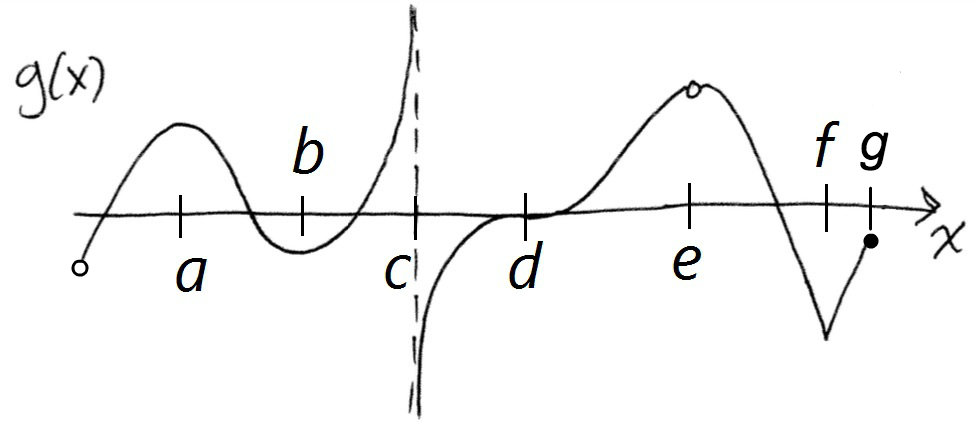
\includegraphics[width=3.3in]{biggraph.jpg}
\end{center}
\begin{solution}
  Critical points: \(a,b,d,f,g\). Local extrema: \(a,b,f\).
\end{solution}
But what if we didn't know what the graph looked like? How would we identify these points?

\textbf{1st Derivative Test:} If $p$ is a critical point of $f$ and $f$ is continuous at $p$, then, moving from left to right, if:
\begin{itemize}
\item \(f'\) changes from positive to negative at \(p\), then
  \fillin[\(p\) is a local minimum][8cm]
\item \(f'\) changes from negative to positive at \(p\), then
  \fillin[\(p\) is a local maximum][8cm]
\end{itemize}
An \textbf{inflection point} of a function $g$ is a point in the
domain of $g$ at which $g$ is continuous and where \fillin[\(g\)
changes concavity][6cm].  Identify any inflection points in the graph below.

\begin{center}
	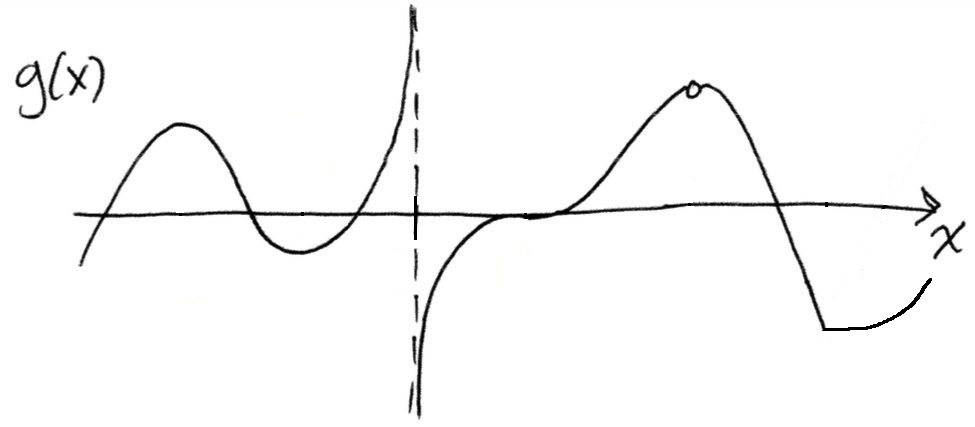
\includegraphics[width=3.3in]{biggraph2.jpg}
\end{center}
But what if we did not know what the graph looked like? How would we identify these points?  
\vspace{0.2in}
\begin{questions}
  \question
    \begin{parts}
    \part Find the location of all local maxima and minima of
      $f(x)=(x^2-4)^7$.  Justify using calculus -- \textit{this means
        you cannot just use a graph of f.}
    \part Find the location of any inflection points of $f(x)=(x^2-4)^7$.  Justify using calculus.
    \end{parts}
    \begin{solution}
      \begin{enumerate}[(a)]
      \item We first compute \(f'(x) = 7(x^2-4)^6 2x\). Then, we check
        \begin{itemize}
        \item \(f'(x) = 0\): at \(x=-2, 0, 2\)
        \item \(f'(x)\) DNE: none
        \end{itemize}
        Then, we make a sign line by checking test points
        \begin{itemize}
        \item \(f'(-3) = 14(-3)(9-4)^6 < 0\)
        \item \(f'(-1) = 14(-1)(1-4)^6 < 0\)
        \item \(f'(1) = 14(1)(1-4)^6 > 0\)
        \item \(f'(3) = 14(3)(9-4)^6 > 0\)
        \end{itemize}
        This gives us sign line:
\begin{tikzpicture}
\node at (-0.5,0) {\(f'\)};
\draw (0,0)--(4,0);
\node at (.5,.2) {-};
\node at (1,-.4) {$-2$};
\draw (1,-.1)--(1,.1);
\node at (1.5,.2) {-};
\node at (2,-.4) {$0$};
\draw (2,-.1)--(2,.1);
\node at (2.5,.2) {+};
\node at (3,-.4) {$2$};
\draw (3,-.1)--(3,.1);
\node at (3.5,.2) {+};
\end{tikzpicture}

From this, we can conclude that \(f\) has a local minimum at \(x=0\).
\item We first compute \(f''(x) = 14(x^2-4)^6+14x \cdot 6(x^2-4)^5 2x
  = 14(x^2-4+12x^2)(x^2-4)^5 = 14(13x^2-4)(x^2-4)^5\). Note that this factors as \(f''(x) =
  14(\sqrt{13}x-2)(\sqrt{13}x+2)(x^2-4)^5\). Then, we check
  \begin{itemize}
  \item \(f''(x) = 0\): at \(x=-2,-\frac{2}{\sqrt{13}},\frac{2}{\sqrt{13}},2\)
  \item \(f''(x)\) DNE: none
  \end{itemize}
  Then, we make a sign line by checking test points
  \begin{itemize}
  \item \(f''(-3) = 14(13(-3)^2-4)((-3)^2-4)^5 > 0\)
  \item \(f''(-1) = 14(13(-1)^2-4)((-1)^2-4)^5 < 0 \)
  \item \(f''(0) = 14(13(0)^2-4)((0)^2-4)^5 > 0\)
  \item \(f''(1) = 14(13(1)^2-4)((1)^2-4)^5 < 0\)
  \item \(f''(3) = 14(13(-3)^2-4)((-3)^2-4)^5 > 0\)
  \end{itemize}
        This gives us sign line:
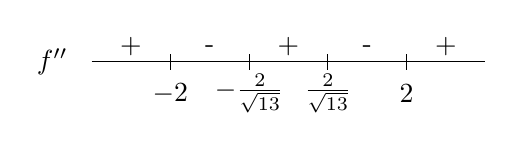
\begin{tikzpicture}
\node at (-0.5,0) {\(f''\)};
\draw (0,0)--(5,0);
\node at (.5,.2) {+};
\node at (1,-.4) {$-2$};
\draw (1,-.1)--(1,.1);
\node at (1.5,.2) {-};
\node at (2,-.4) {$-\frac{2}{\sqrt{13}}$};
\draw (2,-.1)--(2,.1);
\node at (2.5,.2) {+};
\node at (3,-.4) {$\frac{2}{\sqrt{13}}$};
\draw (3,-.1)--(3,.1);
\node at (3.5,.2) {-};
\node at (4,-.4) {$2$};
\draw (4,-.1)--(4,.1);
\node at (4.5,.2) {+};
\end{tikzpicture}

From this, we conclude \(f\) has inflection points at \(x=-2,-\frac{2}{\sqrt{13}},\frac{2}{\sqrt{13}},2\).
      \end{enumerate}
    \end{solution}
   \question Give an example of
\begin{enumerate}[(a)]
	\item a function $f$ and a critical point $a$ for $f$ such that $f$ \emph{does not} have a local maximum or a local minimum at $x=a$.
	\item a function $f$ and a value of $a$ such that $f'(a)=f''(a)=0$ but $f$ \emph{does not} have an inflection point at $a$.
\end{enumerate}
\begin{solution}
  \(f(x) = x^3\) is a solution for both (a) if \(a=0\). \(f(x) = x^4\)
  is a solution for (b) if \(a=0\).
\end{solution}
   \question Find and justify using calculus the location of all local maxima and minima of $$h(x)= \left\{
\begin{array}{ll}
      e^x & x\leq 0 \\
      x^4-4x+1& 0 < x %< 2 \\
      %\displaystyle \frac{1}{(x-4)^2} & x\geq 2
\end{array} 
\right.
$$ 
\begin{solution}
  We compute \[
    h'(x) =
    \begin{cases}
      e^x & x < 0\\
      4x^3 - 4 & 0 < x
    \end{cases}
  \]
  Note that \(h\) is not differentiable at \(x=0\).
  We then check
  \begin{itemize}
  \item \(h'(x) = 0\): at \(x=1\)
  \item \(h'(x)\) DNE: at \(x=0\)
  \end{itemize}
  Then, we make a sign line by checking
  \begin{itemize}
  \item \(h'(-1) = e^{-1} > 0\)
  \item \(h'(0.5) = \frac{1}{2}-4 = -3.5 < 0\)
  \item \(h'(2) = 32-4 = 28 > 0\)
  \end{itemize}
  This gives us the sign line:
\begin{tikzpicture}
\node at (-0.5,0) {\(h'\)};
\draw (0,0)--(3,0);
\node at (.5,.2) {+};
\node at (1,-.4) {$0$};
\draw (1,-.1)--(1,.1);
\node at (1.5,.2) {-};
\node at (2,-.4) {$1$};
\draw (2,-.1)--(2,.1);
\node at (2.5,.2) {+};
\end{tikzpicture}

Thus, \(h\) has a local maximum at \(x=0\) and a local minimum at \(x=1\).
\end{solution}
\question Find all critical points of $$p(x) = x^3(x^2-5x+5), \quad \textrm{given that}$$ $$p'(x) =5x^2(x-1)(x-3) \quad \textrm{and} \quad p''(x) = 10x(2x^2-6x+3).$$

Then \textbf{use concavity} to determine whether the $p$ has a local max or min at each critical point, if possible.  This is called the \textbf{2nd Derivative Test}.
\begin{solution}
  From this information, we have
  \begin{itemize}
  \item \(p'(x) = 0\): at \(x=0,1,3\)
  \item \(p'(x)\) DNE: none
  \end{itemize}
  Then, we compute
  \begin{itemize}
  \item \(p''(0) = 0 \implies\) the 2nd derivative test is inconclusive.
  \item \(p''(1) = 10(2-6+3) = -10 < 0 \implies p\) has a local
    maximum at \(x=1\).
  \item \(p''(3) = 30(18-18+3) = 90 > 0 \implies p\) has a local
    minimum at \(x=3\).
  \end{itemize}
\end{solution}
\question Suppose that the \textit{derivative} of an everywhere differentiable function $k(x)$ is given by $$k'(x) = (x-a)(x-b)(x-c),$$ where $a<b<c$ are constants.  Using calculus, find the location of all local maxima and minima.
  \begin{solution}
    We see that
    \begin{itemize}
    \item \(k'(x) = 0\): at \(x=a,b,c\)
    \item \(k'(x)\) DNE: none
    \end{itemize}
    Furthermore, we can use ``sign logic'' to determine the sign line:

\begin{tikzpicture}
\node at (-0.5,0) {\(k'\)};
\draw (0,0)--(8,0);
\node at (1,.2) {\(\scriptstyle - \cdot - \cdot - = -\)};
\node at (2,-.4) {$a$};
\draw (2,-.1)--(2,.1);
\node at (3,.2) {\(\scriptstyle + \cdot - \cdot - = +\)};
\node at (4,-.4) {$b$};
\draw (4,-.1)--(4,.1);
\node at (5,.2) {\(\scriptstyle + \cdot + \cdot - = -\)};
\node at (6,-.4) {$c$};
\draw (6,-.1)--(6,.1);
\node at (7,.2) {\(\scriptstyle + \cdot + \cdot + = +\)};
\end{tikzpicture}

From here, we can determine \(k\) has a local minimum at \(x=a\) and
\(x=c\) and a local maximum at \(x=b\).
  \end{solution}
\question (Winter 2018 Exam 2) % problem 4
In the following question, use calculus to justify your answers and show enough evidence to
demonstrate that you have found them all. Determine your answers algebraically.
\begin{enumerate}[(a)]
\item Let $f(x)$ be a continuous function defined for all real numbers with derivative given by
$$f'(x)=\frac{(2x+1)(x-2)^2}{(x+3)^{\frac{1}{3}}}.$$
Find the $x$-coordinate(s) of the local maximum(s) and local minimum(s) of the function $f(x)$. Write \emph{none} if the function has no local maximum(s) and/or local minimum(s).
\item Let $g(x)$ be a continuous function defined for all real numbers with second derivative given by
$$g''(x)=(2^x-4)(x^2-4).$$
Find the $x$-coordinates of the inflection points of the function $g(x)$. Write \emph{none} if the function has no inflection points.
\end{enumerate}
\begin{solution}
  See \href{https://dhsp.math.lsa.umich.edu/exams/115exam2/w18/s4.pdf}{https://dhsp.math.lsa.umich.edu/exams/115exam2/w18/s4.pdf}
\end{solution}
\question (Fall 2017 Final Exam) % problem 7
	Let $A$ and $B$ be positive constants and $f(x) = \frac{A(x^2-B)}{\sqrt{x-3}}$ for all $x>3$. Note that
	$$f'(x)=\frac{A(x^2-12x+B)}{2(x-3)^{\frac{3}{2}}} \qquad \textrm{and} \qquad f''(x)=\frac{2A(x^2-8x+24-B)}{4(x-3)^{\frac{5}{2}}}.$$
	Find all the values $A$ and $B$ such that $f$ has an inflection point at $(8,2)$. Use calculus to justify that $(8,2)$ is an inflection point. If there are no such values, write \emph{none}.
        \begin{solution}
          See \href{https://dhsp.math.lsa.umich.edu/exams/115exam3/f17/s7.pdf}{https://dhsp.math.lsa.umich.edu/exams/115exam3/f17/s7.pdf}
        \end{solution}
      \question (Winter 2018 Exam 2) % problem 5
        The graph of the function $f$ with domain $-4 \leqslant x \leqslant 8$ is shown below. The function $f(x)$ satisfies:
\begin{itemize}
\item $f(x) = 1.5 x^{\frac{1}{3}}$ for $-1<x<1$, and
\item $f(x) = 4 +\displaystyle\sin \left( \frac{\pi}{4} (x-3) \right)$ for $3 \leqslant x < 5$ and $5 < x \leqslant 8$.
\end{itemize}
\vspace{-0.5em}
\begin{center}
  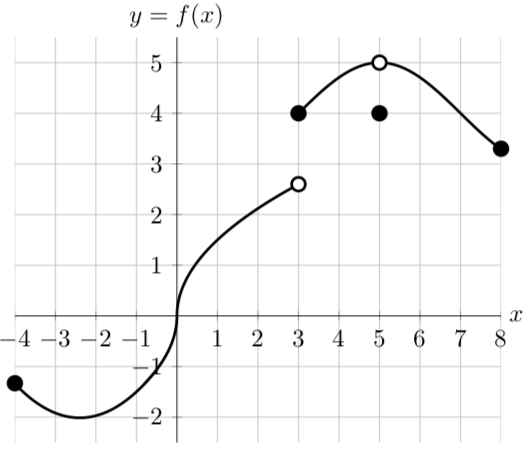
\includegraphics[scale=0.4]{Exam2W2018Problem5}
\end{center}
\begin{enumerate}[(a)]
	\item Estimate the $x$-coordinate(s) of all the local minimum(s) of $f(x)$ in $-4<x<8$. Write \emph{none} if $f(x)$ does not have any local minima.
	\item Find the value(s) of $b$ in $-4<x<8$ for which the limit $\displaystyle\lim_{h \rightarrow 0} \frac{f(b+h)-f(b)}{h}$
does not exist. Write \emph{none} if there are no such values of $b$.
 	\item Estimate the $x$-coordinate(s) of all critical points of $f(x)$ in $-4 < x < 8$. Write \emph{none} if $f(x)$ does not have any critical points.
\end{enumerate}
\begin{solution}
  See \href{https://dhsp.math.lsa.umich.edu/exams/115exam2/w18/s5.pdf}{https://dhsp.math.lsa.umich.edu/exams/115exam2/w18/s5.pdf}
\end{solution}
      \question (Winter 2017 Exam 2) % problem 1
        The graph of a portion of the derivative of $b(x)$ is shown below. Assume that $b(x)$ is defined and continuous on $[-5, 6]$.
        \begin{center}
          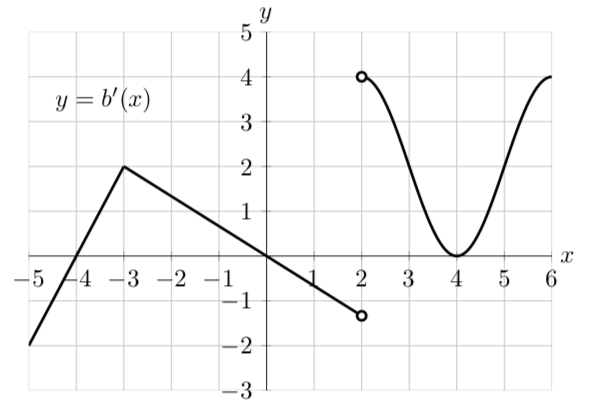
\includegraphics[scale=0.4]{Winter2017Exam2Problem1}
        \end{center}
\begin{enumerate}[(a)]
	\item At which of the following values of $x$ does $b(x)$ appear to have a critical point?
		$$x=-4 \qquad x=-3 \qquad x=2 \qquad x=3 \qquad \textrm{none of these}$$
	\item At which of the following values of $x$ does $b(x)$ attain a local minimum?
	$$x=-4 \qquad x=2 \qquad x=3 \qquad x=5 \qquad \textrm{none of these}$$
	\item At which of the following values of $x$ does $b(x)$ appear to have an inflection point?
	$$x=-3 \qquad x=2 \qquad x=3 \qquad x=5 \qquad \textrm{none of these}$$
	\end{enumerate}
        \begin{solution}
          See \href{https://dhsp.math.lsa.umich.edu/exams/115exam2/w17/s1.pdf}{https://dhsp.math.lsa.umich.edu/exams/115exam2/w17/s1.pdf}
        \end{solution}
\question (Fall 2016 Exam 2) % problem 6
	The entire graph of a function $g(x)$ is shown below. Note that the graph of $g(x)$ has a horizontal tangent line at $x = 1$ and a sharp corner at $x = 4$.
        \begin{center}
          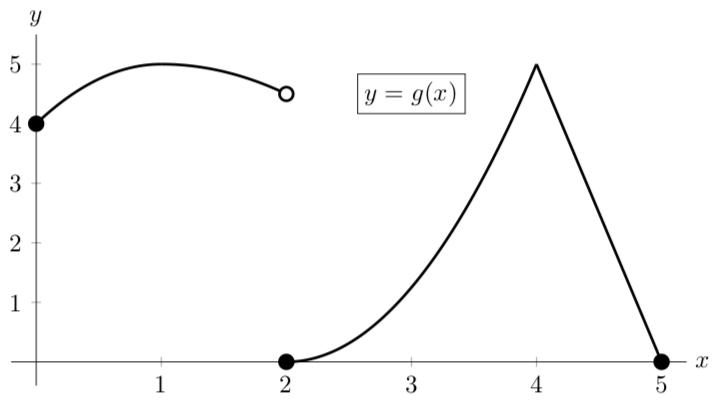
\includegraphics[scale=0.5]{Fall2016Exam2Problem6}
        \end{center}
\begin{enumerate}[(a)]
	\item At which of the following values of $x$ does $g(x)$ appear to have a critical point?		
	$$x=1 \qquad x=2 \qquad x=3 \qquad x=4 \qquad \textrm{none of these}$$
	\item At which of the following values of $x$ does $g(x)$ attain a local maximum?
	$$x=1 \qquad x=2 \qquad x=3 \qquad x=4 \qquad \textrm{none of these}$$
	\end{enumerate}
        \begin{solution}
          See \href{https://dhsp.math.lsa.umich.edu/exams/115exam2/f16/s6.pdf}{https://dhsp.math.lsa.umich.edu/exams/115exam2/f16/s6.pdf}
        \end{solution}
\question (Winter 2016 Exam 2) % problem 4
	Let $h(x)$ be a twice differentiable function defined for all real numbers $x$. (So $h$ is differentiable and its derivative $h'$ is also differentiable.)
Some values of the derivative of $h$ are given in the table below.
\begin{center}
  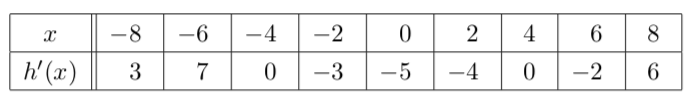
\includegraphics[scale=0.5]{Winter2016Exam2Problem4}
\end{center}
\begin{enumerate}[(a)]
\item Circle all the intervals below in which $h(x)$ must have a critical point.
$$-8 < x < -6  \qquad -6 < x < 2 \qquad -2 < x < 2 \qquad 2 < x < 6 \qquad 6 < x < 8 \qquad \textrm{none of these}$$
\item Circle all the intervals below in which $h(x)$ must have a local extremum (i.e. a local maximum or a local minimum).
$$-8 < x < -6  \qquad -6 < x < -2 \qquad -2< x < 2 \qquad 2 < x < 6 \qquad 6< x < 8 \qquad \textrm{none of these}$$
\item Circle all the intervals below in which $h(x)$ must have an inflection point.
$$-8 < x < -4  \qquad -4 < x < 0 \qquad 0 < x < 4 \qquad 2 < x < 6 \qquad 4 < x < 8 \qquad \textrm{none of these}$$
\end{enumerate}
\begin{solution}
  See \href{https://dhsp.math.lsa.umich.edu/exams/115exam2/w16/s4.pdf}{https://dhsp.math.lsa.umich.edu/exams/115exam2/w16/s4.pdf}
\end{solution}
\end{questions}
\end{document}
%%% Local Variables:
%%% mode: latex
%%% TeX-master: t
%%% End:
